%\newpage % sonst formatierung im arsch 
\subsection{Untersuchung des Hall-Effekts bei Kupfer}
\label{sec:aufgabe_b}

Die Hallspannung ist grundlegend von zwei Werten abhängig. Dem \textbf{Magnetfeld} und dem Strom $\symup{I_q}$ durch den die Elektronen eine Geschwindigkeit $\bar{v_{d}}$ erhalten. %eventuell Verweise
Im Folgen haben wir jeweils einen Wert konstant bei hoher Spannung gehalten, für möglichst aussagende Ergebnisse, und das Verhalten jeweils untersucht. 
Zudem differenzieren wir zwischen positiver und negativer Polung, um die Messungenauigkeiten die den Geräten verschuldet sind, im späteren Verlauf zu reduzieren. % mehr Gründe hier.
Wir finden also zwei Abbildung, die sich sehr ähnlich sind. Für den genauen Wert der Spannung bedienen wir uns anschließend dem Zusammenhang \cite[9]{V311.pdf} 
\begin{align*}
\symup{U_{ges+}}&= \symup{U_{h}} + \symup{U_{stör}} \\
\symup{U_{ges-}}&= - \symup{U_{h}} + \symup{U_{stör}}
\end{align*}
\begin{equation}
\label{eq:ugesamt}
\symup{U_{H}}= \frac{1}{2}(\symup{U_{ges+}} -\symup{U_{ges-}})
\end{equation}

Sowohl $\symup{U_{ges+}}$ als auch $\symup{U_{ges-}}$ sind uns durch die Messungen bekannt, also können wir nun die Hall-Spannung ohne Störspannung sowohl 
ausrechnen als auch darstellen.

\subsubsection{konstantes Magnetfeld}
\label{sec:Auswertung_bconst}
Die ersten Messungen wurden mit konstantem Magnetfeld durchgeführt. In unserem Fall lag der Strom $\symup{I_b}$, welcher den Elektromagneten betrieben hat bei konstanten $4.6\si{\ampere}$.
Der variable Teil kommt also durch den Strom $\symup{I_q}$ hinzu welcher bei $0\si{\ampere}$ beginnt und von uns vor jeder neuen Messung um $0.5\si{\ampere}$ erhöht wurde.
\\ %komisches layout von lateX, kp was da los ist
\begin{figure}[!h]
   \centering
    \includegraphics[width=\textwidth]{"build/u_hall.pdf"}
    \caption{iq variabel, Bfeld const\\Fehler für mT $\pm$ 0.0005\\Fehler für $I_b \pm 0.001$}
    \label{fig:Uhall}
\end{figure}

Der Graph wird durch ein Polynom dritten Grades dargestellt, verläuft aber annähernd linear in beide Polrichtungen. Auffallend ist die Verschiebung auf der Y-Achse %Grund 
welche keinen Physikalischen Hintergrund hat. Also lässt sich diese als Fehler bewerten und gilt zu zukünftiger Beachtung in kommenden Rechnungen.
Die Verschiebung lässt sich errechnen in dem man die Werte für $\symup{I_b}=0$ des Polynoms sucht, welches durch folgende Funktion gegeben wird.  
Die Parameter sind mit jeweiligen Fehler im Anhang aufgeführt.  

\paragraph{Positive Polung}
\begin{equation}
   \symup{U_{ges+}}(\symup{I_q})=-0.000006 \cdot \symup{I_q}^3 + 0.000112\cdot\symup{I_q}^2 + 0.001876 \cdot\symup{I_q} + 0.000727 
\end{equation}

\paragraph{Negative Polung} 
\begin{equation}
   \symup{U_{ges-}}(\symup{I_q})=-(-0.000047 \cdot \symup{I_q}^3 + 0.000280\cdot\symup{I_q}^2 -0.002408\cdot\symup{I_q} + 0.000084)
\end{equation}

%Die Nullstelle für den verschobenen Part der postiven Polung lässt durch einsetzten von $0$ bestimmen und sieht wie folgt aus:
%
%\begin{align}
%   \symup{m\si{\tesla}}(0)&=-0.000006 \cdot 0^3 + 0.000112 \cdot 0^2 + 0.001876 \cdot 0 + 0.000727 \\
%   \symup{m\si{\tesla}}(0)&=0.000727
%\end{align}
%
%Der Graph ist also um $0.000727$ $\symup{\si{\volt}}$ nach oben verschoben.
%Was in der Auswertung und berechnung von anderen Werten berücksichtigt werden muss.

%auswertung ugesamt mit der formel
Es liegen uns also jetzt beide Auswertungen $\symup{U_{ges+}}$ und $\symup{U_{ges-}}$ die wir als nach \eqref{eq:ugesamt} folgende Darstellung abbilden können.
 % was leider nicht passt lol... !!!!!!!!!!!!!

\begin{figure}[h]
   \centering
   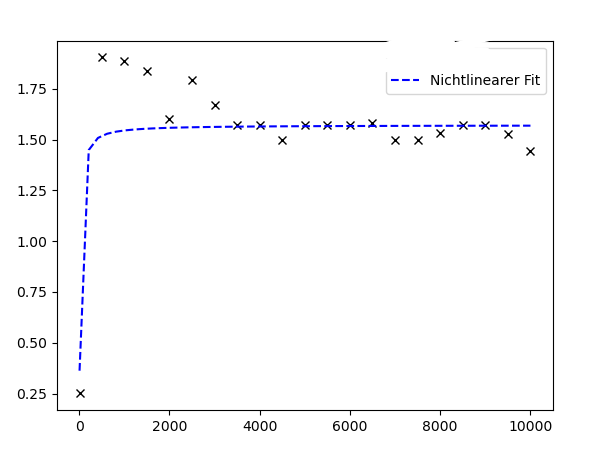
\includegraphics[width=\textwidth]{build/plot1.pdf} %achsen beschriften, werte prüfen!
   \caption{$\symup{U_h}$ als Überschneidung beider Pole}
   \label{fig:auswertunghall}
\end{figure}

Hier wird noch kein Fehler mit einbezogen, der durch die Messung entstanden ist. man kann den Graphen bloß als eine Art Annährung werten. 
Es bietet sich an mit Python den Fehler jeweils für die gemessenen Werte ausrechnen zu lassen und als Tabelle auszugeben.


\subsubsection{konstanter Strom $\symup{I_q}$}
\label{sec:Auswertung_iconst}

Diese abbildende  Kurve der \textbf{Hallspannung} steht in Abhängigkeit zum Strom $\symup{I_b}$ der durch den Elektromagneten fließt und somit ein Magnetfeld erzeugt.
Der Graph ist deutlich stärker Gekrümmt als \ref{fig:Uhall} und wird wieder durch ein Polynom dritten Grades abgebildet. 


\begin{figure}
   \centering
    \includegraphics[width=\textwidth]{"build/u_hall_i.pdf"}
    \caption{iq const, Bfeld variabelt$\pm$ 0.0005\\Fehler für $I_b \pm 0.001$}
    \label{fig:Uhall}
 \end{figure}



Dieses mal mit der Funktion analog zu \ref{sec:Auswertung_bconst}
\paragraph{Positive Polung}


\begin{equation}
   \symup{U_h}(\symup{I_b})=-0.000146 \cdot \symup{I_b}^3 + 0.001047\cdot\symup{I_b}^2 -0.000053\cdot\symup{I_b} -0.000740
\end{equation}

\paragraph{Negative Polung}

\begin{equation}
   \symup{U_h}(\symup{I_b})=-0.000044 \cdot \symup{I_b}^3 + 0.000415\cdot\symup{I_b}^2 -0.003241\cdot\symup{I_b} 0.000137
\end{equation}

\begin{figure}[!h]
   \centering
   \includegraphics[width=\textwidth]{build/plot2.pdf} %achsen beschriften
   \caption{$\symup{U_h}$ als Überschneidung beider Pole}
   \label{fig:auswertunghall}
\end{figure}

Auffallend ist die Darstellung. Diese wurde mit einem Polynom dritten Grades geplottet was eigentlich gegen die physikalischen Zusammenhänge
spricht. Diese beschreiben nämlich die Spannung als linearen Wachstum, also ein Polynom ersten Grad. Im Verlauf der Auswertung wird der Graph durch einen linearen $fit$
in Python auf ein Grad reduziert um so den physikalischen Bedingungen gerecht zu werden.


%Tabelle einfügen.

%Tabelle mit weerten aus ugesamt 
%\begin{tabel}
%
%\end{tabel}